\chapter[Embasamento Teórico]{Embasamento Teórico}
\section{Modelagem Matemática} 

A modelagem matemática pode ser feita de três formas a partir dos modelos caixa branca, cinza e preta, o primeiro necessita de bastante informação sobre o sistema, utilizando equações determinísticas, submodelos detalhados e entendimento físico. Enquanto que o modelo caixa preta, é realizado unicamente a partir de dados obtidos por meio da inserção de sinais controlados no sistema. Por último, o modelo caixa cinza é o meio termo entre os modelos caixa branca e preta, no qual é utilizado o entendimento físico do sistema e os dados obtidos \cite{barbosa2010}. Todas as três categorias de modelos possibilitam a descrição de um sistema físico utilizando funções matemáticas. Normalmente essa funções são Equações Diferenciais Ordinárias (EDO), as quais expressam as diferenças entre os estados em função de uma variável \cite{witelski2015}, como por exemplo o tempo. 

Várias metodologias são utilizadas para a facilitar a obtenção das equações diferenciais, como: modelagem por compartimentos, a qual tem como finalidade separar o sistema em segmentos menores e descrevê-los por meio da transmissão de materiais ou energia (\citeauthor{anderson2013compartmental}, \citeyear{anderson2013compartmental}; \citeauthor{King2011}, \citeyear{King2011}). Outra forma é a modelagem análoga, que tem como objetivo realizar uma analogia entre a dinâmica real e um domínio mais familiar para o indivíduo que está realizando o processo de modelagem \cite{Khoo2000}, um exemplo é a aplicação da lei de Ohm na representação análoga de modelos biológicos, como na Figura~\ref{exemplo_analogo1} é a  representação análoga elétrica da mecânica linear do músculo. Sendo assim, a variável $F_o$ representa o elemento contráctil do músculo, o resistor ($R$) simboliza os tendões e os capacitores ($Cs$ e $Cp$) descrevem o tecido conjuntivo.

\begin{figure}[htb]
 \begin{center}
  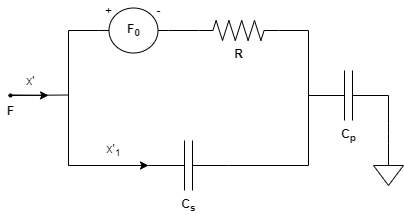
\includegraphics[width=3.0in]{figuras/linear_musculo.png}
  %\vspace{-15pt}
   \caption{{Modelo Elétrico Análogo do Músculo. Adaptado de \cite{Khoo2000}}}
   \label{exemplo_analogo1} 
  \end{center}
\end{figure}

Outro exemplo é a metodologia \textit{Bond Graph} (BG), que emprega uma representação gráfica de um sistema embasada em conceitos como troca e fluxo de energia e iterações entre as diferentes grandezas físicas do modelo (\cite{Rosa2014}; \cite{DeOliveira2016}) incluindo magnitudes dos domínios elétrico, mecânico, hidráulico e pneumático \cite{garcia}, a Figura~\ref{exemplo_bg1} exemplifica uma modelagem BG do olho humano.

\begin{figure}[htb]
 \begin{center}
  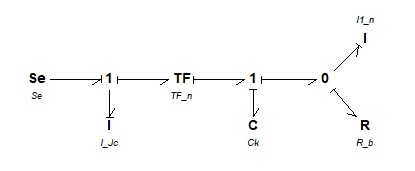
\includegraphics[width=4.0in]{figuras/olho_diabetico.jpg}
  %\vspace{-15pt}
   \caption{{Modelo BG do olho humano (Adaptado do artigo)}}\label{exemplo_bg1}
  \end{center}
\end{figure}

A partir da modelagem completa, os modelos são utilizados para várias propostas, como: análise de comportamento dinâmico, projeto metódico de sistema, seleção de parâmetros para se alcançar estados específicos, projeto de controladores para automatização de processos ou do próprio sistema, estabilidade e adequação do comportamento do sistema (\citeauthor{Aguirre2004}, \citeyear{Aguirre2004}; \citeauthor{Kypuros2013}, \citeyear{Kypuros2013}). Muitas vezes, a modelagem matemática é utilizada em sistemas biológicos, visando analisar o comportamento do corpo em diferentes cenários, muitas vezes não homeostáticos \cite{DeOliveira2016}. Além do mais, busca-se compreender os efeitos e adequação de sistemas endógenos e exógenos (\citeauthor{Rosa2013}, \citeyear{Rosa2013}; \citeauthor{Rosa2014}, \citeyear{Rosa2014}). 

\section{Metodologia Bond Graph}

Inventado em 1954 \cite{borutzky2011}, o Bond Graph é um método gráfico para modelagem e simulações, o qual retrata sistemas considerando a descrição da troca de energia ou informações entre componentes de diferentes domínios de energia, como: elétrico, hidráulico, mecânico (translação e rotação), térmico, magnético e químico (\cite{Rosa2013}; \cite{balthazar}; \cite{Alabakhshizadeh2011}). Associa-se os elementos do sistema físico a estruturas de junção, que retratam restrições para o mesmo \cite{gawthrop}, permitindo a conversão do sistema em uma representação em espaço de estados. Além do mais, a metodologia BG  foi desenvolvida para facilitar a derivação sistemática de EDOs que regem a resposta dinâmica do modelo em análise.

O Bond Graph é um gráfico orientado (dígrafo), desta forma sua estrutura é puramente topológica \cite{borutzky2017bond}. É um dígrafo, pois as ligações dos elementos são feitas com setas mostrando o caminho em que o par fluxo/esforço percorre, as principais variáveis utilizadas são esforço (e), fluxo (f), momento (p) e deslocamento(q), a tabela \ref{tab:Variaveis_bg_eletronicos} exemplifica essas variáveis para circuitos elétricos, as quais foram aplicadas ao longo deste documento  (\cite{borutzky2011}). %\cite{kypuros2013system};\cite{RosaTIBIA}).

\begin{table}[H]
\centering
    \caption{Variáveis para Circuitos Elétricos}
    \label{tab:Variaveis_bg_eletronicos}
        \begin{tabular}{|c|c|c|}
        \hline
        \textbf{Variável Generalizada} & \textbf{Variável Elétrica} & \textbf{Unidade} \\ \hline
        Esforço (e) & Voltagem ($\mu$) & \(Volt(V) = \frac{(N \cdot m)}{C}\) \\ \hline
        Fluxo (f) & Corrente (i) & \(Ampere(A) = \frac{C}{s}\) \\ \hline
        Momento (p) & Fluxo magnético($\omega$) & \(Wb = V \cdot s\) \\ \hline
        Deslocamento (q) & Carga(q) & \(C = A \cdot s\) \\ \hline
    \end{tabular}
\end{table}

Por conseguinte, as portas do BG são os locais em que os subsistemas podem ser interconectados, o que permite que o fluxo de energia. Além disso, para a modelagem dos sistemas foi definida um conjunto básico de elementos multiportas, esses elementos servem como representação matemática dos componentes básicos dos sistemas físicos \cite{karnopp2012system}, utilizando esses modelos básicos é possível realizar a modelagem dos efeitos físicos de sistemas mais complexos. Portanto, adequando-se as variáveis gerais e os elementos multiportas é possível modelar uma grande variedade de domínios de energia. Os elementos são divididos de forma geral em: uma porta, duas portas e multiportas.

\subsection{Elementos de uma porta} \label{sec:1_porta}
Um elemento de uma porta (elementos passivos), como o próprio nome já evidencia só tem uma porta de energia, existindo um único par de esforço/fluxo \cite{karnopp2012system}, os elementos mais básicos de uma porta são diferenciados pela forma de funcionamento: dissipar energia (elemento R), armazenar energia potencial (elemento C), armazenar energia cinética (elemento I). 


\begin{itemize}
    \item \textbf{Elemento R:} \\
    A utilização desse elemento é para a perda da energia do sistema \cite{borutzky2009bond}, por exemplo resistores elétricos que convertem a energia elétrica em calor \cite{dorf}. A equação \ref{eq:resistor_1} demonstra a relação constitutiva do elemento R básico idealizado, equação essa que relaciona diretamente esforço e fluxo como uma função estática.

    \begin{equation}
        \label{eq:resistor_1}
        e = r\cdot f 
    \end{equation}

    A tabela \ref{tab:resistor} demonstra essa relação  ao domínio geral e elétrico e os elementos R básicos desses domínios.

    \begin{table}[H]
    \centering
        \caption{Resistor no Domínio Elétrico}
        \label{tab:resistor}
            \begin{tabular}{| c | c | C{2.5cm} | C{2cm} | C{3cm}|}
            \hline
            \textbf{Domínio} & \textbf{Parâmetros} & \textbf{Unidade} & \textbf{Símbolo Padrão} & \textbf{Símbolo BG}\\ \hline
            Geral & \begin{minipage}[c][11mm][c]{.12\textwidth}
            \vspace{1mm} \(R = \frac{e}{f}\) \end{minipage} & N/A & -  & - \\ \hline
        
            Elétrico & R, resistência & Ohms ($\Omega$) & \begin{minipage}[c][11mm][c]{.12\textwidth}
            \vspace{1mm} 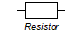
\includegraphics[width=\linewidth, height=10mm]{figuras/Embasamento/resistor.png}\label{fig:res}
            \end{minipage} & \begin{minipage}[c][11mm][c]{.12\textwidth}
            \vspace{1mm} 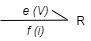
\includegraphics[width=\linewidth, height=7mm]{figuras/Embasamento/BG_resistor.png}\label{fig:BG_res}
            \end{minipage} \\ \hline
        \end{tabular}
    \end{table}
    
    \item \textbf{Elemento C} \\
    Esse tipo de elemento tem uma relação constitutiva entre esforço e deslocamento. Como falado anteriormente, o elemento tipo C é caracterizado por armazenamento de energia potencial, o nome C então vem de capacitância ou complacência, desta forma assumindo a linearidade do componente, a equação \ref{eq:capacitor_1} é a equação geral dos elementos C.

    \begin{equation}
        \label{eq:capacitor_1}
        e = \frac{q}{C} 
    \end{equation}

    Porém, o BG realiza relações de energia para isso é necessário a associação fluxo/esforço, esta é dada pela equação \ref{eq:capacitor_2}, pela causalidade derivativa, ou pela equação \ref{eq:capacitor_3}, causalidade integrativa.

    \begin{equation}
        \label{eq:capacitor_2}
        f = \frac{dq}{dt} = \frac{d (C \cdot e)}{dt}
    \end{equation}

    \begin{equation}
        \label{eq:capacitor_3}
        e = \frac{q}{C} = \int f \frac{dt}{C}
    \end{equation}

    A tabela \ref{tab:capacitor} demonstra os elementos C básico do domínio Elétrico.

    \begin{table}[H]
    \centering
        \caption{Capacitor no Domínio Elétrico}
        \label{tab:capacitor}
            \begin{tabular}{| c | c | C{2.5cm} | C{2cm} | C{3cm}|}
            \hline
            \textbf{Domínio} & \textbf{Parâmetros} & \textbf{Unidade} & \textbf{Símbolo Padrão} & \textbf{Símbolo BG}\\ \hline
            Geral & $C = \frac{q}{e}$ & N/A & - & -  \\ \hline
        
            Elétrico & C, capacitância & Farad (F) & \begin{minipage}[c][11mm][c]{.12\textwidth}
            \vspace{1mm} 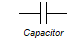
\includegraphics[width=\linewidth, height=10mm]{figuras/Embasamento/capacitor.png}\label{fig:cap}
            \end{minipage} & \begin{minipage}[c][11mm][c]{.12\textwidth}
            \vspace{1mm} 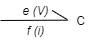
\includegraphics[width=\linewidth, height=7mm]{figuras/Embasamento/BG_capacitor.png}\label{fig:BG_cap}
            \end{minipage}  \\ \hline
        \end{tabular}
    \end{table}

    \item \textbf{Elemento I} \\
    Enquanto os elementos C relacionam esforço e deslocamento, elementos I relacionam momento e fluxo. A equação \ref{eq:indutor_1}, caracteriza de forma ideal e linear os elementos I, nota-se uma similaridade com a equação \ref{eq:capacitor_1}, I é o parâmetro inercial e para novamente se obter uma equação \(e X f\), utilizamos a definição de momento \(p = e \cdot dt\), equação \ref{eq:indutor_2}.

    \begin{equation}
        \label{eq:indutor_1}
        f = \frac{p}{I} 
    \end{equation}
    
    \begin{equation}
        \label{eq:indutor_2}
        f = \int e dt = \frac{d (If)}{dt} 
    \end{equation}

    \begin{table}[H]
    \centering
        \caption{Indutor no Domínio Elétrico}
        \label{tab:indutor}
            \begin{tabular}{| c | c | C{2.5cm} | C{2cm} | C{3cm}|}
            \hline
            \textbf{Domínio} & \textbf{Parâmetros} & \textbf{Unidade} & \textbf{Símbolo Padrão} & \textbf{Símbolo BG}\\ \hline
            Geral & $I = \frac{p}{f}$ & N/A & - & -  \\ \hline
        
            Elétrico & L, indutância & Henry (H) & \begin{minipage}[c][11mm][c]{.12\textwidth}
            \vspace{1mm} 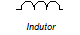
\includegraphics[width=\linewidth, height=10mm]{figuras/Embasamento/indutor.png}\label{fig:ind}
            \end{minipage} & \begin{minipage}[c][11mm][c]{.12\textwidth}
            \vspace{1mm}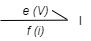
\includegraphics[width=\linewidth, height=7mm]{figuras/Embasamento/BG_indutor.png}\label{fig:BG_ind}
            \end{minipage}  \\ \hline
        \end{tabular}
    \end{table}
    
    
    \item \textbf{Tetraedro de estados}\\
    Uma forma de entender como cada elemento de uma porta se relaciona com as variáveis é por meio da analise da Figura~(\ref{fig:tetraedro}), onde os vértices são as variáveis de potência e energia e as arestas descrevem a relação funcional entre essas variáveis chaves e, f, p, q (\cite{karnopp2012system}; \cite{Kypuros2013})

    \begin{figure}[ht]
        \centering
        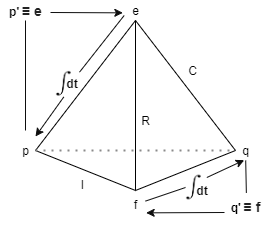
\includegraphics[scale=0.7]{figuras/tetraedro.png}
        \caption{Tetraedro de Estados (redesenhado  a partir de Paynter (1961) e Karnopp, Margolis, and Rosenberg (2000)).}
        \label{fig:tetraedro}
    \end{figure}
\end{itemize}


\subsection{Elemento de duas portas}
Existem dois tipos básicos de elemento duas portas, os quais são subsistemas que não podem ser modelados usando os elementos básicos de uma porta, os elementos básicos de duas portas são: os giradores (GY) e os transformadores(TF). Esses elementos têm como características a transmissão de energia entre elementos do sistema, também servindo para interfacear domínios de energia diferente.

\begin{itemize}
    \item \textbf{Elementos Giradores}
    Os giradores transmitem energia, a relação é dada pela equação~\ref{eq: giradores}, onde nota-se que a relação é realizada entre esforço e fluxo, sendo r o módulo do girador que indica a relação entre o esforço de um lado com o fluxo do outro.
    
    \begin{equation}\label{eq: giradores}
        e_x = r\cdot f_y 
    \end{equation}


    \item \textbf{Elementos Transformadores}
    Estes elementos diferentemente dos giradores, tem a relação fluxo com fluxo ou esforço com esforço, o módulo do transformador n indica a relação proporcional entre os esforços ou fluxos. A equação \ref{eq: transformadores} descreve a relação entre esforços e fluxos para o transformador:
    
    \begin{equation}\label{eq: transformadores}
        e_x = m_x \cdot e_y
    \end{equation}
\end{itemize}


\subsection{Elementos multiportas}
Os elementos multiportas (Junção) permitem a conexão de elementos e subsistemas de domínios distintos. Da mesma forma que, os elementos de junção são responsáveis pela implementação da lei de conservação  de energia, uma vez que a energia não é dissipada nem armazenada. Sendo assim, esses elementos podem ser divididos em: Junção esforço comum e Junção fluxo comum. A partir da  conservação da energia interna, é possível escrever a seguinte equação:

\begin{equation}
    \label{eq:juncoes}
    e_1 \cdot f_1 +  e_2 \cdot f_2 + ... +e_n \cdot f_n = 0
\end{equation}

\begin{itemize}
    \item \textbf{Junção Esforço Comum}
    A junção de esforço comum ou também conhecida por Junção-0, é um ponto de encontro para várias ligações de energia com esforços iguais, conforme a equação~\ref{eq:juncao_0}. Além do mais em circuitos eletrônicos, a junção-0 representa componentes em paralelo.
 
    \begin{equation}\label{eq:juncao_0}
        e_1(t) = e_2 (t) = ... = e_n (t)
    \end{equation}

    E consequentemente, a partir da lei de conservação de energia na equação~\ref{eq:juncoes}, pode-se determinar as relações dos fluxos conforme a fórmula~\ref{eq:juncao_0_1} a soma dos fluxos é igual a zero:

    \begin{equation}\label{eq:juncao_0_1}
        f_1 (t) +  f_2  (t) + ... + f_n (t) = 0
    \end{equation}

\item \textbf{Junção Fluxo Comum }
    A junção de fluxo comum ou também conhecida por Junção-1, é um ponto de encontro para várias ligações de energia com fluxos iguais, segui.  Além do mais em circuitos eletrônicos, a junção-1 representa componentes em série.

    \begin{equation}\label{eq:juncao_1}
        f_1(t) = f_2 (t) = ... = f_n (t)
    \end{equation}

    Sendo assim, a soma dos esforços é igual zero:

    \begin{equation}\label{eq:juncao_1_1}
        e_1 (t) +  e_2  (t) + ... + e_n (t) = 0
    \end{equation}
\end{itemize}


\section{Análise de Sistemas}
\subsection{Função de Transferência}
A Função de Transferência (FT) é uma função que relaciona algebricamente a saída de um sistema à sua entrada. Consequentemente, essa relação permite separar entrada, saída e sistema. Da mesma forma, é possível realizar a convergência união das relações matemáticas dos subsistemas para uma representação total do sistema \cite{nise}. Além do mais, qualquer sistema físico representado por uma equação diferencial linear invariante no tempo pode ser modelado como uma função de transferência. Do mesmo modo, uma FT pode ser descrita como a razão entre as transformadas de Laplace da saída e da entrada, como na equação~\ref{ft_geral1}, onde $x(t)$ é a entrada e $y(t)$ a saída do sistema e $H(s)$ a função de transferência. 	


\begin{equation}\label{ft_geral1}
    H(s) = \frac{Y(s)}{X(s)} = \frac{\mathcal{L}\{y(t)\}}{\mathcal{L}\{x(t)\}}
\end{equation}

Deve-se notar que a equação \ref{ft_geral1} é geral para um sistema sem condições iniciais, e se a entrada for um impulso unitário, a FT será a resposta do sistema no domínio da frequência, $H(s) = Y(s)$ \cite{Khoo2000}. É importante lembrar que as funções de transferência só podem ser definidas para sistemas lineares e estacionários \cite{dorf} e uma descrição por meio de FT não inclui informações da estrutura interna do sistema, podendo sistemas diferentes terem a mesma FT, até mesmo de diferentes domínios de energia. 

As funções de transferência tem uma importância muito grande para análise do comportamento estático e dinâmico do sistema. Sendo assim, a partir da aplicação metodologias de análise, como a análise dos polos e zeros da FT do sistema pode-se simplificar o cálculo da resposta do mesmo~\cite{nise}.

\subsubsection{Polos e Zeros}

A partir da Equação Diferencial Ordinária (EDO) generalizada de ordem $n$ conforme a equação \ref{eq: ft_generica} é possível determinar os polos e zeros da função.

\begin{equation}\label{eq: ft_generica}
    \frac{d^ny(t)}{dt^n} + q_{n-1}\frac{d^{n-1}y(t)}{dt^{n-1}} +\cdot\cdot\cdot+q_0y(t) =
    \frac{d^mx(t)}{dt^m} + p_{m-1}\frac{d^{m-1}x(t)}{dt^{m-1}} +\cdot\cdot\cdot+p_0x(t) 
\end{equation}

A função de transferência resultante, a partir da equação~\ref{eq: ft_generica}, é apresentada na equação~\ref{ft_geral2}. O polinômio denominador é nomeado de polinômio característico do sistema e dessa forma, o grau $n$ é a ordem do sistema e suas raízes são os polos ou valores em que a função de transferência se torne infinita. Já o polinômio numerador não recebe nome específico, e suas raízes ou valores em que a função de transferência se torne igual a zero são os denominadas zeros. O sistema é causal se o número de polos for maior que zeros,  $n>m$, determinando assim que a saída $y(t_0)$ não depende de uma entrada $x(t)$ para $t>t_0$.

\begin{equation}
G(s) = \frac{p^m + p_{m-1}s^{m-1}+\cdot\cdot\cdot+p_0}{s^n + q_{n-1}s^{n-1} +\cdot\cdot\cdot+q_0} \label{ft_geral2}
\end{equation}

O gráfico de polos e zeros é capaz de esboçar graficamente o caráter da resposta transitória do sistema, é importante notar que caso os polos estejam do lado direito do eixo $j\omega$ o sistema será instável. Outrossim, a partir da equação de transferência com substituição de valores encontrados a partir dos polos e zeros do sistema é possível determinar características do sistema, como: tempo de subida, tempo de acomodação subamortecido, amortecido, criticamente amortecido, superamortecido.


\subsection{Espaço de Estados}

A representação por meio do espaço de estados é um método unificado para modelar, analisar e projetar uma vasta variedade de sistemas, assim como é possível representar sistemas não lineares e com condições iniciais não nulas (\cite{nise}; \cite{Aguirre2004}). A simplicidade da representação em espaço de estados está na possibilidade de representar uma EDO de n-ésima ordem com uma simples matriz diferencial de primeira ordem.

O estado de um sistema descrito por uma EDO no instante zero é determinado pelas condições iniciais, podendo considerar entrada, saída e sinais internos do sistema, caracterizando o estado a cada instante de tempo. A partir dos valores das variáveis de estados e do sinal de entrada é possível calcular a saída no próximo instante de tempo \cite{keviczky2019control}. 

A representação em espaço de estados é composta por duas equações matriciais a \textbf{equação de estados} e a \textbf{equação de saída} conforme demonstrado no diagrama de blocos da figura \ref{fig_db_estados}. As dimensões das matrizes dependem da ordem do sistema, quantidade de entradas e de saídas do sistema.


\begin{figure}[htb]
 \begin{center}
  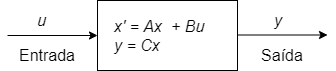
\includegraphics[width=2.5in]{figuras/Embasamento/fig_espaco_estados.png}
  %\vspace{-15pt}
   \caption{{Diagrama de Blocos do Espaço de Estados}}\label{fig_db_estados}
  \end{center}
\end{figure}

\subsubsection{Equação de Estados}

A equação de estados, equação~\ref{eq: espaco_estados0} , representa a variação de estados do sistema ($\dot{x}(t)$) que é a relação entre o vetor de estados ($x(t)$) e o vetor de entradas do sistema ($u(t)$). 

\begin{equation}\label{eq: espaco_estados0}
    \dot{x}(t) = Ax(t){~}+{~}Bu(t) 
\end{equation}

O vetor de estados é composto por componentes do sistema que são variáveis no tempo, como por exemplo os elementos C e I do Bond Graph na secção~\ref{sec:1_porta}. As condições iniciais de um sistema é dada pelos valores de $x(t)$, no instante $t_0$. Dessa forma, $A$ e $B$, são matrizes constantes, dando peso às variáveis de estado e entradas do sistema de acordo com as necessidades do vetor de variação de estados.

Para um sistema de ordem $n$, com $i$ entradas a equação~\ref{eq: espaco_estados0} expandida será:

\begin{equation}\label{eq: estados_expandida0}
\left[ \begin{matrix}
    \dot{x}_1 \cr \dot{x}_2 \cr  \vdots \cr \dot{x}_n 
\end{matrix} \right]
=  
\left[ \begin{matrix} 
A_{(1,1)} & A_{(1,2)} & \cdots  & A_{(1,n)}\cr
A_{(2,1)} & A_{(2,2)} & \cdots  & A_{(2,n)}\cr
\vdots    & \vdots    & \ddots  & \vdots   \cr
A_{(n,1)} & A_{(n,2)} & \cdots  & A_{(n,n)}\cr
\end{matrix} \right] \cdot
\left[ \begin{matrix}
    x_1 \cr x_2 \cr  \vdots \cr x_n 
\end{matrix} \right] +
\left[ \begin{matrix} 
B_{(1,1)} & B_{(1,2)} & \cdots  & B_{(1,i)}\cr
B_{(2,1)} & B_{(2,2)} & \cdots  & B_{(2,i)}\cr
\vdots    & \vdots    & \ddots  & \vdots   \cr
B_{(n,1)} & B_{(n,2)} & \cdots  & B_{(n,i)}\cr
\end{matrix} \right] \cdot
\left[ \begin{matrix}
    u_1 \cr u_2 \cr  \vdots \cr u_i 
\end{matrix} \right] 
\end{equation}

\subsubsection{Equação de Saída}

A equação de saída, equação~\ref{eq: espaco_estados1}, apresenta a relação entre estados e entradas do sistema para gerar as $j$ saídas do sistema.

\begin{equation} \label{eq: espaco_estados1}
     y(t) = Cx(t){~}+{~}Du(t)
\end{equation}

Abaixo verifica-se a versão expandida da equação de saída:

\begin{equation}\label{eq: estados_expandida1}
\left[ \begin{matrix}
    y_1 \cr y_2 \cr  \vdots \cr y_j 
\end{matrix} \right]
=  
\left[ \begin{matrix} 
C_{(1,1)} & C_{(1,2)} & \cdots  & C_{(1,n)}\cr
C_{(2,1)} & C_{(2,2)} & \cdots  & C_{(2,n)}\cr
\vdots    & \vdots    & \ddots  & \vdots   \cr
C_{(j,1)} & C_{(j,2)} & \cdots  & C_{(j,n)}\cr
\end{matrix} \right] \cdot
\left[ \begin{matrix}
    x_1 \cr x_2 \cr  \vdots \cr x_n 
\end{matrix} \right] +
\left[ \begin{matrix} 
D_{(1,1)} & D_{(1,2)} & \cdots  & D_{(1,i)}\cr
D_{(2,1)} & D_{(2,2)} & \cdots  & D_{(2,i)}\cr
\vdots    & \vdots    & \ddots  & \vdots   \cr
D_{(j,1)} & D_{(j,2)} & \cdots  & D_{(j,i)}\cr
\end{matrix} \right] \cdot
\left[ \begin{matrix}
    u_1 \cr u_2 \cr  \vdots \cr u_i 
\end{matrix} \right] 
\end{equation}

\subsection{Estabilidade de Sistemas Dinâmicos}

Com a modelagem matemática realizada é possível implementar diversas análises da resposta no tempo e na frequência. Uma das análises mais importantes e mais esclarecedoras do comportamento do sistema é a estabilidade do sistema.

Uma sistema estável apresenta a partir de uma entrada limitada uma saída limitada \cite{dorf}, para sistemas biológicos a estabilidade está diretamente relacionada a homeostase do sistema \cite{Khoo2000}. A estabilidade de um sistema modelado matematicamente está diretamente relacionada à posição de seus polos ou, no caso de modelagem por espaço de estados, a posição dos autovalores da matriz do sistema.

Desta forma, existe a condição necessária e suficiente para um sistema ser estável é que todos os polos da função de transferência do sistema tenham parte real negativa, isto é, estarem localizados no semiplano esquerdo do plano \textit{\textbf{s}}, por tanto, um sistema não é estável se nem todas as raízes estiverem no semiplano esquerdo.

\subsubsection{Lugar Geométrico das Raízes}

Tendo em vista que a posição dos polos do sistema, determinam sua estabilidade e outras características de desempenho, o método do lugar geométrico das raízes é uma ferramenta que facilita análise, já que fornece de forma gráfica, um esboço aproximado que pode pode ser utilizado para adquirir informações sobre à estabilidade e o desempenho do sistema.

A partir da análise do Lugar Geométrico das Raízes é possível determinar como o sistema se comporta, para diferentes valores aplicados as suas constantes, desta forma, caso os polos não satisfaçam a necessidades do projeto é possível realizar ajustes rápidos observando o posicionamento das raízes. Além de ser um método que facilita a análise para sistemas com diferentes ordens \cite{Aguirre2004}.

\section{Equipamentos de proteção individual - Respirador  VESTA}


As precauções padrão (PP) consistem em estratégias efetivas para a prevenção e controle das infecções, em Serviços de Assistência à Saúde (SAS). Dessa forma, os Equipamentos de proteção individual (EPIs) fazem parte das propostas para minimizar os riscos ocupacionais  entre profissionais da área da saúde (PAS), os quais estão diariamente expostos á Materiais Biológicos (MB) no manuseio de equipamentos e artigos contaminados ou sob suspeita de contaminação e nas situações em que tem-se o risco de contato com: sangue, líquidos corpóreos, secreções e excreções. Dessa forma, os EPIs têm como função proteger a pele, as mucosas e roupas do profissional do contato com MB, o qual pode veicular agentes patogênicos \cite{De2006}.

Diante disso, profissionais de saúde estão vulneráveis aos diversos riscos existentes no ambiente laboral \cite{Ribeiro2010}, uma vez que, o vírus SARS-CoV-2 pode ser dispersado por gotículas suspensas no ar, quando pessoas infectadas tossem, espirram ou conversam. Entretanto, a formação de aerossóis e gotículas são diminuídos com a utilização de máscaras não profissionais por pessoas contaminadas \cite{girardi2020}. Assim, máscaras, respiradores e face shields são EPIs que constituem uma barreira protetora  os quais diminuem a exposição e o risco de infecção para os profissionais de saúde e a população em geral. 

Entretanto, a partir da grande demanda por EPIs destinados ao combate a Covid-19, tanto por parte da equipe de saúde pública, quanto da população do país, tem-se presenciado a falta de disponibilidade de EPIs. Por conseguinte, essa situação implica no uso prolongado do equipamento por parte dos PAS e, por consequência, eleva o risco de contaminação. Neste contexto, como iniciativa da Universidade de Brasília criou-se o Projeto Égide,  o qual visa diminuir os impactos epidemiológicos da expansão da transmissão do vírus SARS- CoV-2. 

Assim,  desenvolveu-se o respirador VESTA que segue os moldes dos respiradores N95 classe 2 PFF, de material tecido-não tecido (TNT), com três camadas: uma camada interna, uma camada externa e um camada média com elemento filtrante de nanomateriais, vide figura , o que poderá diminuir a permeabilidade de partículas e favorecer um efeito biocida em relação às máscaras convencionais como a N95. 

\begin{figure}[H]
 \begin{center}
  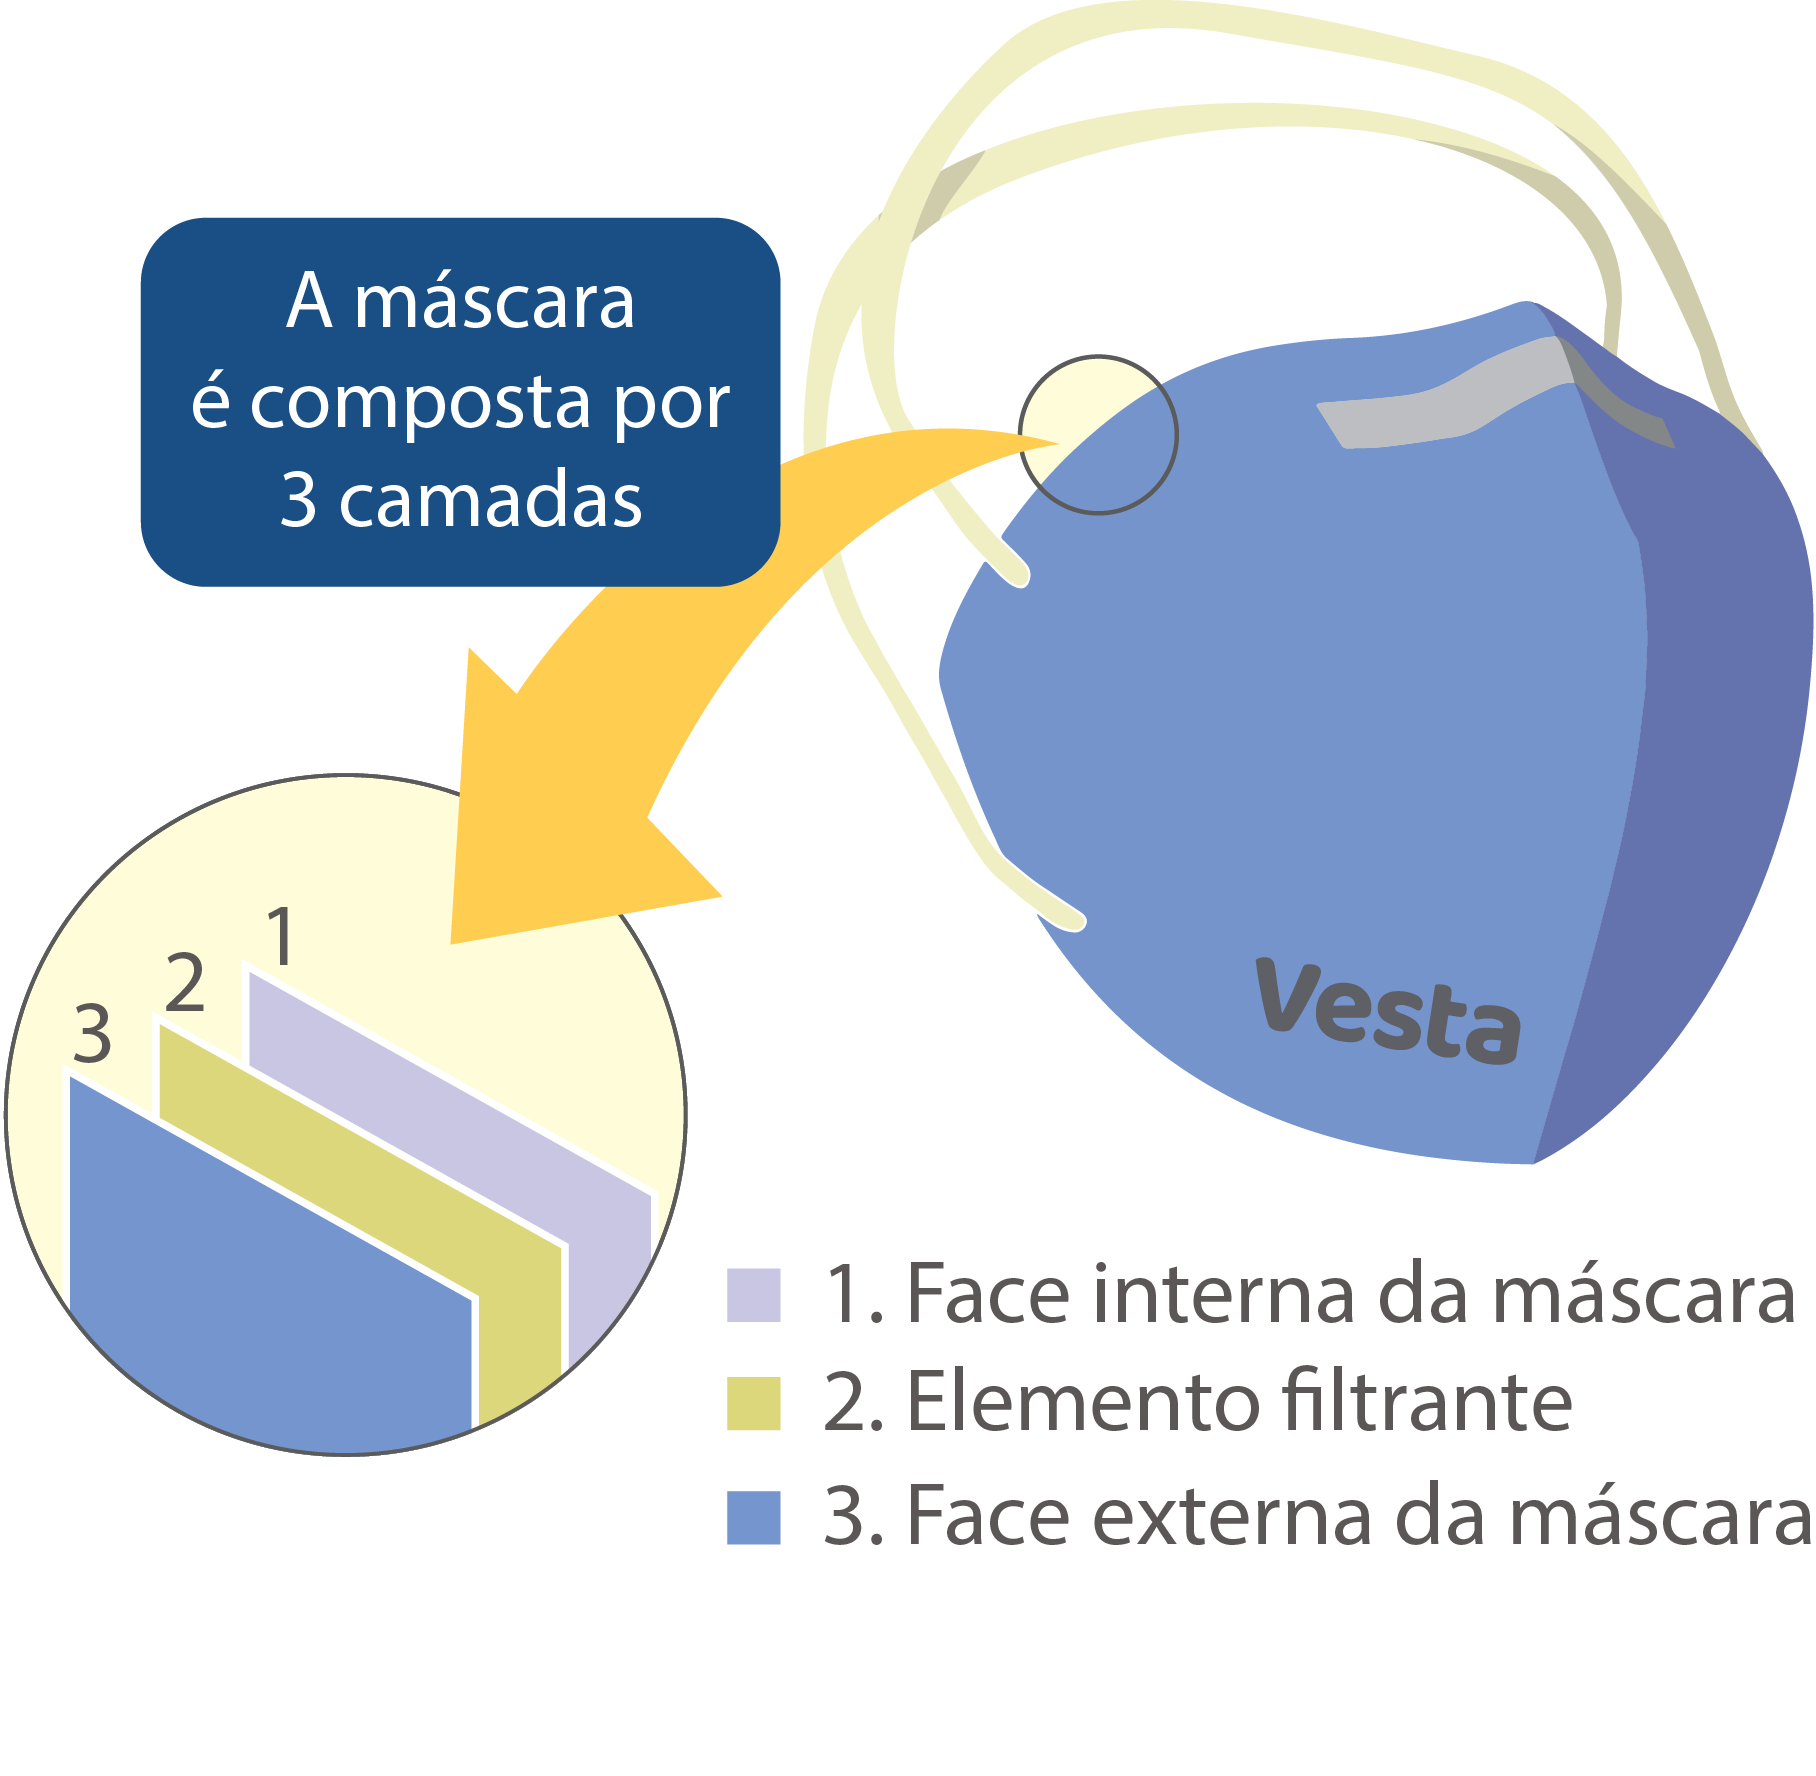
\includegraphics[width=0.4\textwidth]{figuras/Vesta.png}
  %\vspace{-15pt}
   \caption{{Respirador Vesta }}\label{fig:vesta}
  \end{center}
\end{figure}

Sendo assim, escolheu-se a utilização de nanopartículas de quitosana,  devido ao fator atrativo de sua carga catiônica para cargas negativas, como é o caso do vírus SARS-CoV-2, e assim pode atuar como superfície de adsorção e de inativação viral conforme ilustrado na figura  \cite{ciejka}. Dessa forma, o respirador VESTA tem como objetivo ser eficaz contra partículas sólidas e líquidas a base de água e alcançar a inativação dos efeitos nocivos de bactéria e vírus no ambiente hospitalar. 
%citar figura

\subsubsection{Rich Picture}

\subsubsection{5W2H}

\subsection {Elicitação}
A Elicitação de Requisitos é o processo relacionado com as atividades que permitem a compreensão de metas, objetivos e motivos para a construção de um novo sistema de \textit{software} e a identificação de todos os requisitos das partes interessadas que facilitarão o sistema a ser desenvolvido \cite{elliott2012software}. Além disso, as informações coletadas durante a elicitação de requisitos geralmente precisam ser interpretadas, analisadas, modeladas e validadas antes do início da implementação do sistema \cite{nuseibeh2000requirements}.

\subsubsection{Brainstorming}

\subsubsection{Questionário}

\subsubsection{Protótipo de Baixa Fidelidade}

\subsubsection{Storytelling}

\subsubsection{Entrevista}

\subsubsection{Análise de Protocolo}

\subsection {Modelagem}

\subsubsection{Backlog}

\subsubsection{NFR}

\subsubsection{Léxicos}

\subsection {Verificação}

\subsection {Pós-rastreabilidade}

\subsubsection{Priorização (MVP)}

\subsubsection{Backward-from}

\subsection {Rastreabilidade}
A rastreabilidade é um tópico essencial dentro da Engenharia de Requisitos, pois é utilizado para providenciar relações entre requisitos, arquitetura e implementação final do sistema, além de possibilitar uma compreensão dos relacionamentos de dependência entre os requisitos propostos. Dessa forma, a rastreabilidade pode ser implementada como um conjunto de ligações entre os requisitos \cite{sayao2006rastreabilidade}.

A rastreabilidade tem o objetivo de acompanhar e descrever o ciclo de um requisito de duas formas:
\begin{itemize}
    \item Pré-rastreabilidade: documentar o contexto a partir do qual emergem os requisitos;
    \item Pós-rastreabilidade: vincula os requisitos à arquitetura do sistema e sua implementação.
\end{itemize}